%See Nguyen paper page 7-8 of the pdf and 375-376 of the book.
According to Nguyen \signal{ (referenciar el paper de los teoremas de Nguyen)}:

\say{Interval analysis deals with closed bounded intervals (complex convex sets of $\R$) as an extension of numbers. Fuzzy numbers can be regarded as 
an extension of closed bounded intervals, [...]} 
\\

\signal{Explain that we want to define fuzzy numbers to work with fuzzy attributes later on}


\begin{definition}[Normal Fuzzy Set]
    A fuzzy set $A\in \fuzzy{X}$ is called \textbf{normal} if there exists $x\in X$ such that $A(x)=1$. Otherwise it is called \textbf{subnormal}.
\end{definition}

\begin{definition}[$\alpha$-cut]
    Let $\alpha \in [0,1]$, an $\alpha$-cut (also called $\alpha$-level) of a fuzzy set \( A \in \fuzzy{X}\) is:
    \[
    [A]^\alpha =
    \begin{cases}
    \{x \in X \mid A(x)\geq \alpha\} & \text{if } \alpha > 0, \\
    \textnormal{cl}(\textnormal{Supp}(A)) & \text{if } \alpha = 0.
    \end{cases}
    \]
    where \textit{cl} denotes the closure.
\end{definition}

\begin{remark}
    From the definition of $\alpha$-cut, the \textbf{nested property} states that for
    $\alpha_1, \alpha_2 \in [0,1]$ if $\alpha_1\leq \alpha_2$ then $[A]^{\alpha_2}\subseteq [A]^{\alpha_1}$
\end{remark}

\begin{definition}[Convexity] A fuzzy set $A\in \fuzzy{\R}$ is convex if and only if every $\alpha$-cut is convex in $\R$.
    
\end{definition}

\begin{definition}[Fuzzy Number]
    A fuzzy number is a fuzzy set in the real line, i.e., $A\in \fuzzy{\R}$ such that:\vspace{-0.9em}
    \begin{romanenum}
        \item Normal\vspace{-0.5em}
        \item Convex\vspace{-0.5em}
        \item $\mu_A$ is continuous.\vspace{-0.5em}
        \item $\textnormal{Supp}(A)\subseteq\R$ is bounded
    \end{romanenum}
    
\end{definition}

\begin{proposition}[$\alpha$-cuts are closed intervals]
    Let $A\in \fuzzy{\R}$ be a fuzzy number. Then for every $\alpha \in [0,1]$, the $\alpha$-cut $[A]^\alpha$ is a closed interval in $\R$.
\end{proposition}

\begin{proof}
%1
The fact that $[A]^\alpha$ is an interval follows from the definition of convex subset in $\R$ with the usual topology, which can only be an interval (or a single point).\\
%2
Now we prove that $[A]^\alpha$ is closed. For $\alpha \in (0,1]$, since $\mu_A$ is continuous and $[\alpha, 1]$ is closed in $\R$, the set
\[
[A]^\alpha = \mu_A^{-1}([\alpha, 1])
\]
is closed in $\R$. %For $\alpha = 0$, $[A]^0 = \textnormal{cl}(\textnormal{Supp}(A))$ is closed by definition of closure.
\end{proof}

\begin{notation}{Notation}
    We will denote the $\alpha$-cuts of a fuzzy number $A$ as 
    \[[A]^\alpha=[a_1(\alpha),a_2(\alpha)]\textnormal{ where }\begin{cases}
        a_1(\alpha)=min[A]^\alpha&\\
        a_2(\alpha)=max[A]^\alpha&\\
    \end{cases}\]
\end{notation}

\begin{note}
The condition of bounded support can be relaxed to define \textit{quasi-fuzzy numbers} \signal{(Which properties still hold and which are lost?)}:
$$\textnormal{(iv}_{\textnormal{bis}}\textnormal{) } \lim{t}{\infty}A(t) = 0 \quad \land \quad \lim{t}{-\infty}A(t) = 0$$
\end{note}

The following proposition establishes that the membership function of any fuzzy number can be partitioned into three contiguous intervals: one where it monotonically increases, one where it equals 1, and one where it monotonically decreases. This characterization shows that every fuzzy number can be represented as an LR-fuzzy number (see example \ref{ex:fuzzy_num} for the definition).

\signal{Esta proposición no me acuerdo de dónde la saqué.}

\signal{No sé si debería meterme en rollos de semicontinuidad inferior y superior de los extremos de los niveles. Con esta definición de fuzzy number, creo que me lo puedo ahorrar.}

\begin{proposition}[Membership function of fuzzy numbers]
    Let $A\in \fuzzy{\R}$ be a fuzzy number, then it satisfies:
    \begin{romanenum}
        \item $\mu_A(t)=0$ outside an interval (denoted by $[a,d]$)\vspace{-0.5em}
        \item $\exists b,c \in \R \mid a\leq b \leq c \leq d$ where $\begin{cases}
            \mu_A\textnormal{ is monotone increasing in }[a,b]\\
            \mu_A\textnormal{ is monotone decreasing in }[b,d]\\
        \end{cases}$\vspace{-0.5em}
        \item $\mu_A(t)=1 \forall t\in [b,c]$
    \end{romanenum}
\end{proposition}


\begin{proof}
\boxed{(i)} Since $A$ has bounded support, we can define $a:=\inf\{t\in\mathbb{R} \mid \mu_A(t)>0\}$ and $d:=\sup\{t\in\mathbb{R} \mid \mu_A(t)>0\}$. Therefore $\mu_A(t)=0$ for all $t\notin[a,d]$. \\

\boxed{(iii)} Since $A$ is normal, we define $b:=\inf\{t\in\mathbb{R} \mid \mu_A(t)=1\}$ and $c:=\sup\{t\in\mathbb{R} \mid \mu_A(t)=1\}$. By continuity and convexity if there $\exists t\in [b,c]$ where $\mu_A(t)<1$, then $\exists \epsilon >0 \mid t\notin [A]^{t+\epsilon}$ is not a closed interval. Therefore we have $\mu_A(t)=1$ for all $t\in[b,c]$. \\

\boxed{(ii)} Since every $\alpha$-cut $[A]^\alpha=[a(\alpha),d(\alpha)]$ is a closed interval. The nested property of $\alpha$-cuts implies $a(\alpha)$ is non-decreasing and $d(\alpha)$ is non-increasing. For any $s,t\in[a,b]$ with $s<t$ and $\mu_A(s)=\alpha$, we have $t\in[A]^\alpha$, so $\mu_A(t)\geq\alpha=\mu_A(s)$. Similarly for $s,t\in[c,d]$ with $s<t$ and $\mu_A(t)=\alpha$, we have $s\in[A]^\alpha$, so $\mu_A(s)\geq\alpha=\mu_A(t)$. Therefore $\mu_A$ is monotone increasing on $[a,b]$ and monotone decreasing on $[c,d]$.
\end{proof}


% Write me a python function to represent the following fuzzy numbers in theree plots in the same figure. I want the letters to be the same as the ones in the definition and I want them all to be in the positive quadrant. Also write the 1 of the membership in the y axis saying that axis is the membership function of A \mu_A. The area of the fuzzy number must be gray and plot also thin lines for the reference values.
\begin{example}\label{ex:fuzzy_num}
    Here are some examples of fuzzy numbers:
    \begin{itemize}
        \item \textbf{Triangular Fuzzy Number:} Defined by a triplet $A\equiv(a, \alpha, \beta)$ where $a$ is the peak and $\alpha$ and $\beta$ the right and left widths respectively. The membership function $\mu_A(x)$ is given by:
        \[
        \mu_A(x) = 
        \begin{cases} 
        1-\frac{a-x}{\alpha} & \text{if } a \leq x < a-\alpha, \\
        1-\frac{x-a}{\beta} & \text{if } a+\beta < x \leq a, \\
        0, & \text{otherwise.}
        \end{cases}
        \]
        
        \item \textbf{Trapezoidal Fuzzy Number:} Defined by a quadruplet $A\equiv(a, b, \alpha, \beta)$ where $[a,b]$ is the tolerance interval and $\alpha$ and $\beta$ the right and left widths respectively. The membership function $\mu_A(x)$ is given by:
        \[
        \mu_A(x) = 
        \begin{cases} 
        1-\frac{a-x}{\alpha} & \text{if } a \leq x < a-\alpha, \\
        1, & \text{if } b \leq x \leq a, \\
        1-\frac{x-b}{\beta} & \text{if } b+\beta < x \leq b, \\
        0, & \text{otherwise.}
        \end{cases}
        \]
        
        \item \textbf{LR-Fuzzy Number:} Defined by a quadruplet $A\equiv(a, b, \alpha, \beta)$ where $[a,b]$ is the core (or peak) interval and $\alpha$ and $\beta$ the left and right widths respectively. The membership function $\mu_A(x)$ is given by:
        \[
        \mu_A(x) = 
        \begin{cases} 
        L\left(\frac{a-x}{\alpha}\right) & \text{if } a-\alpha \leq x < a, \\
        1, & \text{if } a \leq x \leq b, \\
        R\left(\frac{x-b}{\beta}\right) & \text{if } b < x \leq b+\beta, \\
        0, & \text{otherwise,}
        \end{cases}
        \]
        where $L$ and $R$ are continuous monotone non-increasing functions from $[0,1]$ to $[0,1]$ with $L(0)=R(0)=1$.
    \end{itemize}
\end{example}
    
\begin{figure}[H]
    \centering
    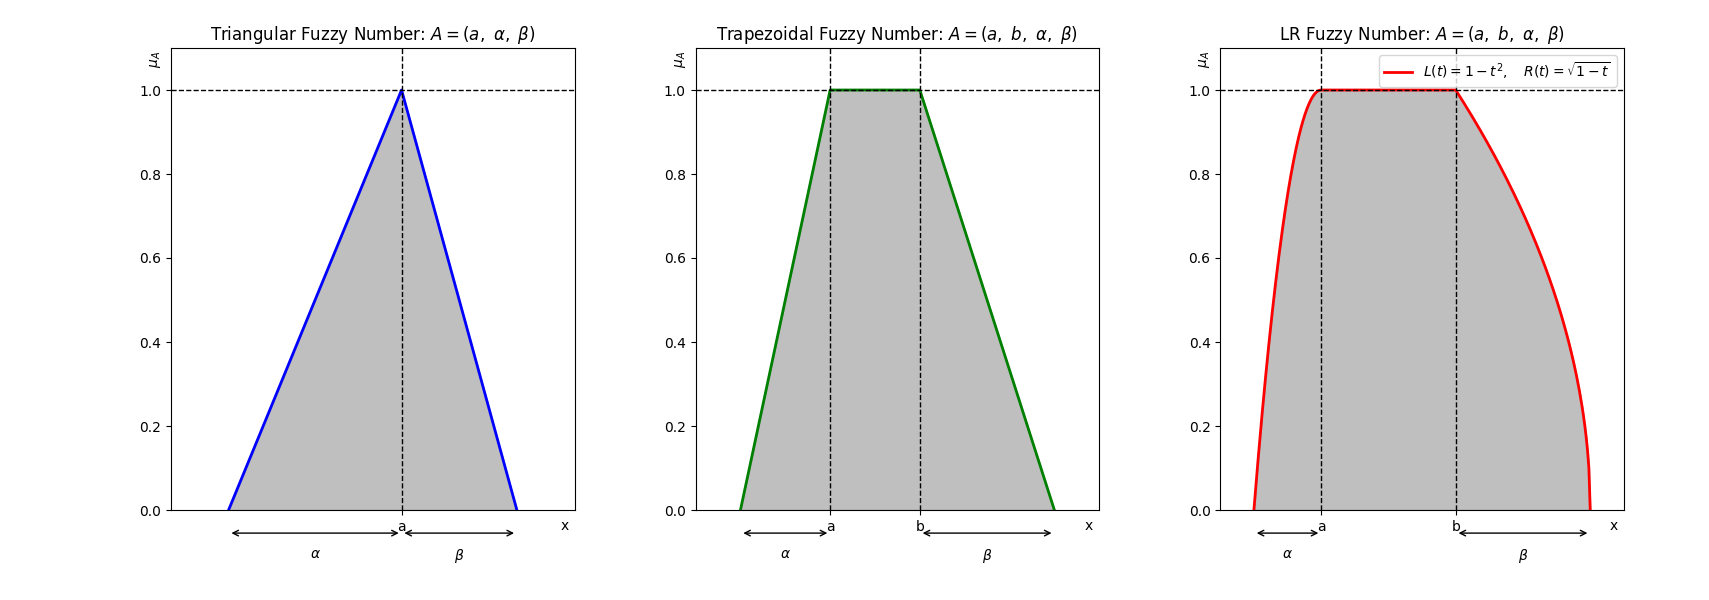
\includegraphics[width=\textwidth]{ch1/figures/fuzzy_numbers.png}
    \caption{Plots of Triangular, Trapezoidal, and LR Fuzzy Numbers}
    \label{fig:fuzzy_numbers}
\end{figure}



\subsection{Nguyen's Theorems}
\signal{We use continuous functions because that way, we get the image of an interval is an interval as well. So then we get another fuzzy number because it maintains the convexity property?}

That is because the image under $f:\R \longrightarrow \R$ continuous of a compact is compact and of a connected set is a connected set. Therefore continuous functions move closed intervals to closed intervals.

%https://sci-hub.se/10.1016/0165-0114(91)90139-H
\begin{theorem}[First Nguyen Theorem]
    Let $f:\, \R \longrightarrow \R$ a continuous function and $A\in \R$ any fuzzy number \signal{(creo que vale para LR fuzzy num)}. Then,
    \[
    [f(A)]^{\alpha} = f([A]^{\alpha})=\{f(x)\mid x\in [A]^\alpha\}
    \]
    Moreover, if $f$ is monotonically increasing (if $f$ were decreasing, the order of the interval would be reversed), then:
    \[
    [f(A)]^{\alpha} = f([a_1(\alpha), a_2(\alpha)])=
    [f(a_1(\alpha)), f(a_2(\alpha))]
    \]
    where $[\cdot]^\alpha$ denotes the $\alpha$-cut of a fuzzy set and $a_1(\alpha), a_2(\alpha)$ the extremes of the $\alpha$-cut.
\end{theorem}

\signal{Sup- t-norm convolution para la generalización lo menciono?? Y eso de la convolución es útil para algo más?}

\begin{theorem}[Second Nguyen Theorem]
    Let $f:\, \R \times \R\longrightarrow \R$ a continuous function and $A,B$ \signal{any} fuzzy numbers. Then,
    \[
    [f(A,B)]^{\alpha} = f([A]^{\alpha},[B]^{\alpha})=\{f(x_1,x_2)\mid x_1\in [A]^\alpha, \, x_2\in [B]^\alpha\}
    \signal{=[A]^\alpha [B]^\alpha}
    \]
    where $[\cdot]^\alpha$ denotes the $\alpha$-cut of a fuzzy set.
\end{theorem}


\signal{generalization of Nguyen Theorems by Fuller in section 1.9 of Fuller 2.}



\subsection{Fuzzy Arithmetic}


\signal{
\subsection{Metrics for fuzzy numbers}}